
%Tipo de documento
\documentclass[a4paper,12pt,twoside]{article} %book, report, letter, beamer


%Paquetes

%Configuracion inicial
\usepackage[utf8]{inputenc}
%\UseRawInputEncoding
\usepackage[spanish]{babel}

%Hipervinculos dinamicos
\usepackage[backref]{hyperref}
%Matematicas
\usepackage{amssymb}
%Comentarios de varias lineas
\usepackage{comment}
%Insertar imagenes
\usepackage{graphicx}
\graphicspath{ {GRAFICAS/} }
%Cuadros de codigo
\usepackage{listings}



% Cuerpo del documento -------------------------------------------------
%Entorno: comando especial que cuenta con parte de incio y de fin.

\begin{document}

%Portada
\begin{titlepage}
\centering

{
\includegraphics[width=0.6\textwidth]{foto_portada.png}\par}
\vspace{1cm}

{\bfseries\LARGE Escuela Técnica Superior de Ingeniería Informática y Telecomunicaciones \par}
\vspace{0.5cm}

{\scshape\Huge Eficiencia de Algoritmos \par}
\vspace{0.5cm}

{\itshape\Large Primera Práctica de Algorítmica \par}
\vfill
{\itshape\Large Doble Grado en Ingeniería Informática y Matemáticas \par}
\vfill

{\Large Autor: \par}
{\Large Leandro Jorge Fernández Vega \par}
\vspace{0.5cm}
{\Large Correo electrónico:}
{\Large leandrofdez@correo.ugr.es \par}
\vfill

{\Large Marzo 2023 \par}

\end{titlepage}

% Crea indice
\tableofcontents
\newpage


\section{Objetivos}


	\begin{itemize}
		\item Conocer en profundidad la importancia de analizar la eficiencia de algoritmos.
		\item Saber contrastar varios tipos de análisis: teórico, empírico e híbrido.
		\item Descubrir algunos de los más frecuentes algoritmos de ordenación y averiguar cómo sacarles el máximo partido.
		\item Aprender a utilizar recursos gráficos como GNUPLOT y aplicar conocimiento estadístico a los análisis.
	\end{itemize}
\newpage


\section{Introducción}

Se plantea la realización de varios análisis de eficiencia sobre diversos algoritmos de ordenación de vectores tipo double: \textit{burbuja, inserción, selección, heapsort, mergesort} y  \textit{quicksort}.\\

Para ello, recurriremos a métodos de análisis teórica, empírica e híbrida, así como ilustraciones gráficas con el propósito de mostrar cada respectiva curva de tiempos.\\

Con esta práctica analizaremos el comportamiento de cada algoritmo en el caso peor, promedio y mejor y veremos qué diferencia supone la compilación con optimización.

\subsection{Datos técnicos del computador utilizado}

\begin{itemize}

	\item Nombre del dispositivo: HP LAPTOP-JNF4H31N

	\item Procesador: 11th Gen, Intel(R) Core(TM) i7-1165G7, 2.80 GHz, 8 núcleos.

	\item RAM instalada: 16,0 GB (15,8 GB usable)

	\item Tipo de sistema: Sistema operativo de 64 bits.

	\item Arquitectura: x86\_64

	\item Cachés: L1d: 192 KiB (4 instances), L1i: 128 KiB (4 instances), L2: 5 MiB (4 instances), L3: 12 MiB (1 instance)

\end{itemize}

  

\subsection{Tipos de análisis a realizar}

\subsubsection{Análisis teórico}

Para determinar a qué orden de eficiencia teórico pertenece un algoritmo consideramos las siguientes definiciones:

\begin{itemize}

	\item Caso Peor:\\
	\begin{math}
	T(n) \in O(f(n)) \Leftrightarrow \exists K \in \mathbb{R^+} , \exists n_0 \in N : T(n) \leq K \cdot{f(n)} \ \ \forall n > n_0 		\end{math}
	
	\item Caso Exacto:\\
	\begin{math}	
	T(n) \in \Theta(f(n)) \Leftrightarrow \exists K \in \mathbb{R^+} , \exists n_0 \in N : T(n) = K \cdot{f(n)} \ \ \forall n > n_0
	\end{math}
	
	\item Caso Mejor:\\
	\begin{math}
	T(n) \in \Omega(f(n)) \Leftrightarrow \exists K \in \mathbb{R^+} , \exists n_0 \in N : T(n) \geq K \cdot{f(n)} \ \ \forall n > n_0
	\end{math}
	
\end{itemize}

\subsubsection{Análisis empírico}

El análisis empírico supone la ejecución del algoritmo de ordenación para diferentes tamaños del vector. Para ello, usaremos los siguientes recursos:\\


\begin{itemize}
	\item La biblioteca $<$chrono$>$ y sus funciones para medir tiempos.
	
	\lstset{language=C++}
	\begin{lstlisting}

#include <chrono>
	
high_resolution_clock::time_point t_antes, t_despues;
duration<double> transcurrido;

t_antes = high_resolution_clock::now();

algoritmo(T, n);

t_despues = high_resolution_clock::now();
transcurrido = 
duration_cast<duration<double>>(t_despues - t_antes);
cout << "el tiempo empleado es " 
<< transcurrido.count() << " s." << endl;
	
	\end{lstlisting}
	

	\item El siguiente script para automatizar la obtención de resultados para diferentes tamaños:

	\lstset{language=Bash}
	\begin{lstlisting}
#!/bin/bash 
#echo "" >> salida.dat
i=tamanio
while [ "$i" -le tamanio_final ]
do
    ./algoritmo $i >> salida.dat
      i=$(( $i + salto ))
done

	\end{lstlisting}
	
\end{itemize}

\newpage
\subsubsection{Análisis híbrido}

Consiste en obtener las constantes ocultas de la función del algoritmo. Para ello, utilizamos la herramienta GNUPLOT. Pondremos como ejemplo un algoritmo cuadrático.\\

Primero deberemos introducir la ecuación de la que queremos obtener los coeficientes:\\

\fbox{gnuplot$>$ f(x) = a0*x*x+a1*x+a2}\\

Después le indicaremos a GNUPLOT que realice un ajuste por mínimos cuadrados, donde \textit{salida.dat} es el fichero de datos.\\

\fbox{gnuplot$>$ fit f(x) 'salida.dat' via a0,a1,a2}\\

La parte que más interesa es el apartado \textit{\textbf{Final set of parameters}}, donde se encuentra el valor de los parámetros.\\

Para graficar utilizamos:\\

\fbox{gnuplot$>$ 'salida.dat', f(x) title 'Curva de Ajuste'}\\

Para determinar la bondad del ajuste, podemos utilizar la varianza, aunque el propio análisis teórico y los resultados gráficos nos permiten confirmar que la ecuación parabólica y n-logarítmica representan buenas aproximaciones para los algoritmos a tratar.


\newpage
%Algoritmos O(n²)

\section{Algoritmos $\textit{O(n²)}$}

Por lo general, los casos peores ocurren cuando se debe ordenar un vector cuyos elementos se encuentran en orden opuesto al criterio de ordenación, los casos promedio cuando los valores se encuentran de forma aleatoria, y los casos mejores cuando el vector ya está ordenado.

\subsection{Burbuja}

	\subsubsection{Peor Caso}
	\begin{itemize}
	
		\item Análisis Teórico:
		
	\lstset{language=C++}
	\begin{lstlisting}
	
void burbuja(double T[], int num_elem)
{
  burbuja_lims(T, 0, num_elem);
};


void burbuja_lims(double T[], int inicial, int final)
{
  int i, j;
  double aux;
  for (i = inicial; i < final - 1; i++)  //O(n)
    for (j = final - 1; j > i; j--)		 //O(n)
      if (T[j] < T[j-1])			 //O(1)
	{
	  aux = T[j];			//O(1)
	  T[j] = T[j-1];
	  T[j-1] = aux;
	}
}

	\end{lstlisting}
	
			Vemos que $T(n) \in O(n^2)$, pues debemos multiplicar cada bucle anidado, cada uno $O(n)$, cuyas operaciones internas son $O(1)$.

\newpage
		\item Análisis Empírico:
		
\begin{table}[h]
	\begin{center}
		\begin{tabular}{|c|c|}
		\hline
		Tamaño & Tiempo \\
		\hline
		5000 & 0.0393354 \\
		10000 & 0.151583 \\
		15000 & 0.336168 \\
		20000 & 0.605485 \\
		25000 & 0.93955 \\
		30000 & 1.34316 \\
		35000 & 1.83589 \\
		40000 & 2.42818 \\
		45000 & 3.0371 \\
		50000 & 3.77297 \\
		55000 & 4.51623 \\
		60000 & 5.3811 \\
		65000 & 6.32231 \\
		70000 & 7.31126 \\
		75000 & 8.40151 \\
		80000 & 9.54319 \\
		85000 & 10.817 \\
		90000 & 12.2579 \\
		95000 & 14.193 \\
		100000 & 14.9369 \\
		105000 & 16.5383 \\
		110000 & 19.058 \\
		115000 & 20.1398 \\
		120000 & 23.533 \\
		125000 & 25.5611 \\
		\hline
		\end{tabular}
	\end{center}
	\caption{Algoritmo Burbuja en caso peor.}
\end{table}
\newpage
			
	
		\item Análisis Híbrido:
		
\begin{figure}[h]
  \begin{center}
  
  	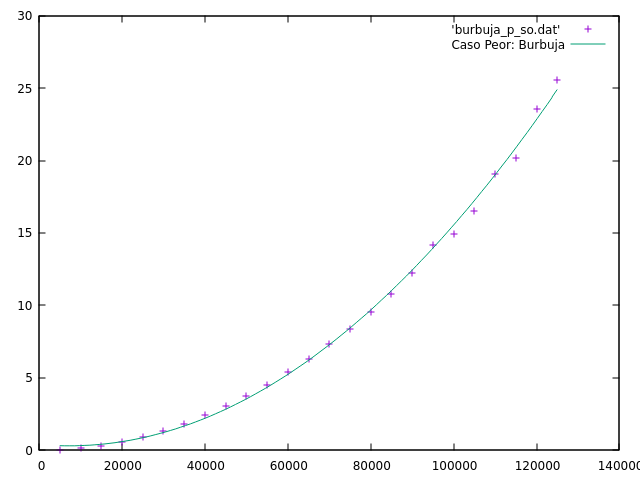
\includegraphics[scale=0.8]{burbuja_p_so_a.png}
  	\caption{Peor: Burbuja ajustada.}
  	
  \end{center}
\end{figure}
		
		
	\end{itemize}
\newpage

	
	\subsubsection{Caso Promedio}

		\begin{itemize}
		\item Análisis Empírico:
		
\begin{table}[h]
	\begin{center}
		\begin{tabular}{|c|c|}
		\hline
		Tamaño & Tiempo \\
		\hline
		5000 & 0.0354 \\
		10000 & 0.1466 \\
		15000 & 0.3824 \\
		20000 & 0.8195 \\	
		25000 & 1.2592 \\
		30000 & 1.8688 \\
		35000 & 2.6216 \\
		40000 & 3.4393 \\
		45000 & 4.3954 \\
		50000 & 5.4516 \\
		55000 & 6.6756 \\
		60000 & 8.7565 \\
		65000 & 10.4434 \\
		70000 & 12.0807 \\
		75000 & 13.8479 \\
		80000 & 15.8711 \\
		85000 & 17.8051 \\
		90000 & 19.9451 \\
		95000 & 22.3192 \\
		100000 & 24.7102 \\
		105000 & 26.0182 \\
		110000 & 27.2127 \\
		115000 & 29.8994 \\
		120000 & 32.4458 \\
		125000 & 35.3310 \\
		\hline
		\end{tabular}
	\end{center}
	\caption{Algoritmo Burbuja en caso promedio.}
\end{table}

\newpage
		\item Análisis híbrido:
		
\begin{figure}[h]
  \begin{center}
  
  	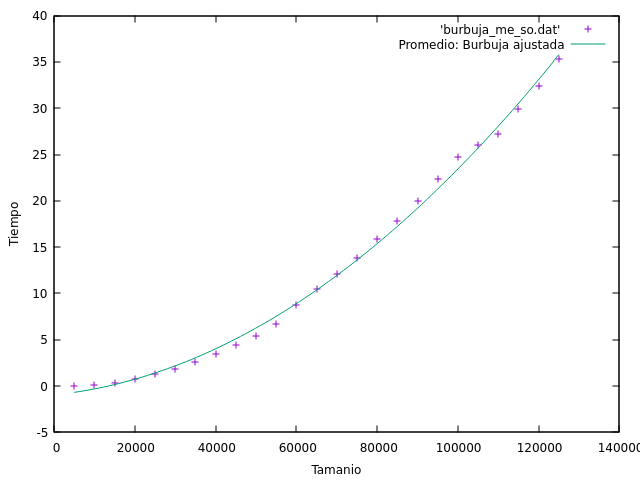
\includegraphics[scale=0.8]{burbuja_me_so_a.png}
  	\caption{Promedio: Burbuja ajustada.}
  	
  \end{center}
\end{figure}
		
		
		
		\end{itemize}
\newpage
	
	\subsubsection{Caso Mejor}
	
		\begin{itemize}
		
		\item Análisis Empírico
		\begin{table}[h]
	\begin{center}
		\begin{tabular}{|c|c|}
		\hline
		Tamaño & Tiempo \\
		\hline
    		5000 & 0.0247754 \\
    		10000 & 0.096502 \\
    		15000 & 0.216596 \\
    		20000 & 0.39421 \\
    		25000 & 0.608742 \\
    		30000 & 0.86785 \\
    		35000 & 1.19753 \\
    		40000 & 1.54282 \\
    		45000 & 1.98436 \\
    		50000 & 2.51476 \\
    		55000 & 3.35318 \\
    		60000 & 3.96248 \\
    		65000 & 4.19091 \\
    		70000 & 4.81067 \\
    		75000 & 5.55205 \\
    		80000 & 6.13531 \\
    		85000 & 6.92302 \\
    		90000 & 7.81883 \\
    		95000 & 10.9967 \\
    		100000 & 12.0232 \\
    		105000 & 11.8855 \\
    		110000 & 12.7667 \\
    		115000 & 14.8504 \\
    		120000 & 15.0451 \\
    		125000 & 16.0888 \\
		\hline
		\end{tabular}
	\end{center}
	\caption{Algoritmo Burbuja en caso mejor.}
\end{table}
\newpage
		
		\item Análisis Híbrido
		
\begin{figure}[h]
  \begin{center}
  
  	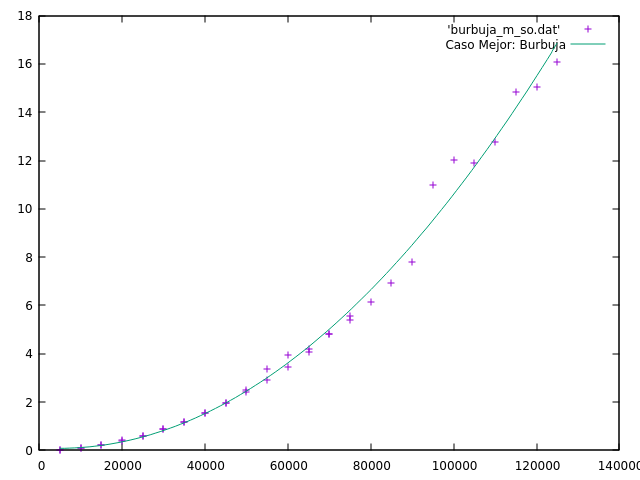
\includegraphics[scale=0.8]{burbuja_m_so_a.png}
  	\caption{Mejor: Burbuja ajustada.}
  	
  \end{center}
\end{figure}
		
		\end{itemize}

\newpage

\subsection{Inserción}

	\subsubsection{Peor Caso}
	\begin{itemize}
	
		\item Análisis Teórico:
		
		\lstset{language=C++}
	\begin{lstlisting}
	
inline static void insercion(double T[], int num_elem)
{
  insercion_lims(T, 0, num_elem);
}


static void insercion_lims(double T[], int inicial, int final)
{
  int i, j;
  int aux;
  for (i = inicial + 1; i < final; i++) { //O(n)
    j = i;
    while ((T[j] < T[j-1]) && (j > 0)) { //O(n)
      aux = T[j];			//O(1)
      T[j] = T[j-1];
      T[j-1] = aux;
      j--;
    };
  };
}

	\end{lstlisting}
	
	Vemos que $T(n) \in O(n^2)$, pues debemos multiplicar cada bucle anidado, cada uno $O(n)$, cuyas operaciones internas son $O(1)$.
	
\newpage

		\item Análisis Empírico:
		
\begin{table}[h]
	\begin{center}
		\begin{tabular}{|c|c|}
		\hline
		Tamaño & Tiempo \\
		\hline
		5000 & 0.0620184 \\
		10000 & 0.242506 \\
		15000 & 0.566694 \\
		20000 & 0.94022 \\
		25000 & 1.46022 \\
		30000 & 2.08983 \\
		35000 & 3.05339 \\
		40000 & 4.16519 \\
		45000 & 5.32819 \\
		50000 & 6.53358 \\
		55000 & 8.23729 \\
		60000 & 11.1729 \\
		65000 & 13.0311 \\
		70000 & 15.3524 \\
		75000 & 17.5375 \\
		80000 & 19.937 \\
		85000 & 22.378 \\
		90000 & 25.1097 \\
		95000 & 28.2986 \\
		100000 & 31.3415 \\
		105000 & 34.0524 \\
		110000 & 34.5518 \\
		115000 & 33.145 \\
		120000 & 34.9532 \\
		125000 & 38.062 \\
		\hline
		\end{tabular}
	\end{center}
	\caption{Algoritmo Inserción en caso peor.}
\end{table}
\newpage
		
\newpage
		\item Análisis Híbrido:
		
\begin{figure}[h]
  \begin{center}
  
  	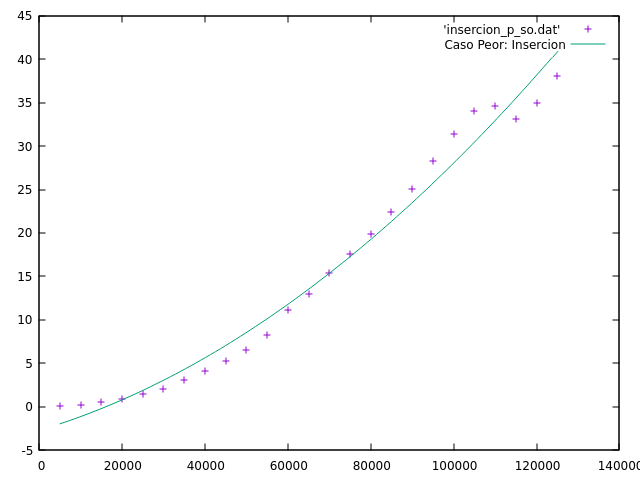
\includegraphics[scale=0.8]{insercion_p_so_a.png}
  	\caption{Peor: Inserción ajustada.}
  	
  \end{center}
\end{figure}
		
	\end{itemize}
	\newpage
	\subsubsection{Caso Promedio}
\begin{itemize}
		
		\item Análisis Empírico
		
\begin{table}[h]
	\begin{center}
		\begin{tabular}{|c|c|}
		\hline
		Tamaño & Tiempo \\
		\hline
		5000 & 0.0297506 \\
		10000 & 0.118948 \\
		15000 & 0.26306 \\
		20000 & 0.462872 \\
		25000 & 0.737131 \\
		30000 & 1.03755 \\
		35000 & 1.41583 \\
		40000 & 1.85352 \\
		45000 & 2.32795 \\
		50000 & 2.87023 \\
		55000 & 3.48715 \\
		60000 & 4.46448 \\
		65000 & 5.42897 \\
		70000 & 6.26744 \\
		75000 & 7.16412 \\
		80000 & 8.10024 \\
		85000 & 9.13163 \\
		90000 & 10.2533 \\
		95000 & 11.398 \\
		100000 & 12.6076 \\
		105000 & 13.8735 \\
		110000 & 15.1217 \\
		115000 & 16.654 \\
		120000 & 18.1177 \\
		125000 & 19.5239 \\
		\hline
		\end{tabular}
	\end{center}
	\caption{Algoritmo Inserción en caso promedio}
\end{table}
\newpage

		\item Análisis Híbrido
		
\begin{figure}[h]
  \begin{center}
  
  	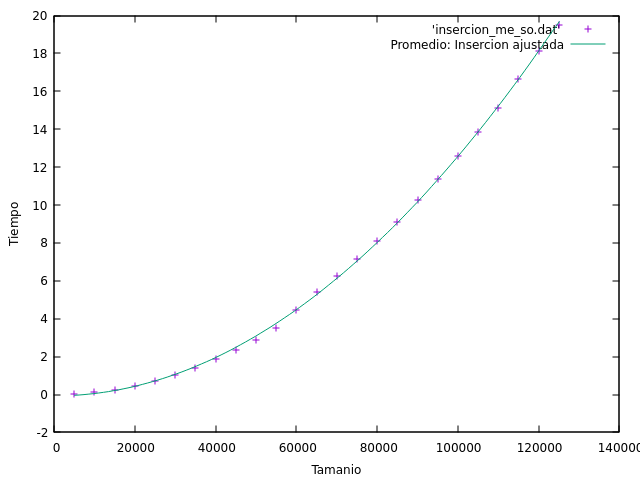
\includegraphics[scale=0.8]{insercion_me_so_a.png}
  	\caption{Promedio: Inserción ajustada.}
  	
  \end{center}
\end{figure}

	\end{itemize}
\newpage
	
	
	\subsubsection{Caso Mejor}
	
	\begin{itemize}
	\item Análisis Empírico
	
	\begin{table}[h]
	\begin{center}
		\begin{tabular}{|c|c|}
		\hline
		Tamaño & Tiempo \\
		\hline
		5000 & 7.855e-06 \\ 
		10000 & 1.4813e-05 \\ 
		15000 & 2.2105e-05 \\ 
		20000 & 3.3938e-05 \\ 
		25000 & 4.5647e-05 \\ 
		30000 & 4.3571e-05 \\ 
		35000 & 5.0524e-05 \\ 
		40000 & 5.762e-05 \\ 
		45000 & 6.6191e-05 \\ 
		50000 & 7.4125e-05 \\ 
		55000 & 7.9946e-05 \\ 
		60000 & 8.72e-05 \\ 
		65000 & 9.7853e-05 \\ 
		70000 & 0.000116023 \\ 
		75000 & 0.000110347 \\ 
		80000 & 0.000117925 \\ 
		85000 & 0.000123104 \\ 
		90000 & 0.000153789 \\ 
		95000 & 0.000165881 \\ 
		100000 & 0.000149033 \\ 
		105000 & 0.000164938 \\ 
		110000 & 0.000165788 \\ 
		115000 & 0.000171772 \\ 
		120000 & 0.000174023 \\ 
		125000 & 0.000184486 \\
		\hline
		\end{tabular}
	\end{center}
	\caption{Algoritmo de Inserción en caso mejor.}
\end{table}
\newpage
	
	\item Análisis Híbrido
\begin{figure}[h]
  \begin{center}
  
  	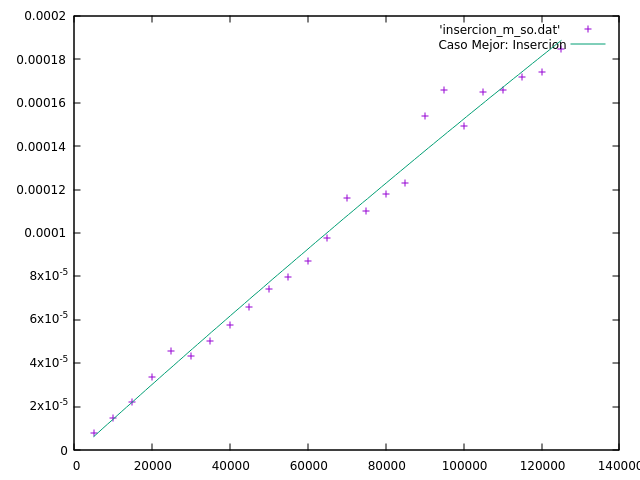
\includegraphics[scale=0.8]{insercion_m_so_a.png}
  	\caption{Mejor: Inserción ajustada.}
  	
  \end{center}
\end{figure}
	
	\end{itemize}
\newpage

\subsection{Selección}

	\subsubsection{Peor Caso}
	\begin{itemize}
	
		\item Análisis Teórico:
		
		\lstset{language=C++}
	\begin{lstlisting}
	
void seleccion(double T[], int num_elem)
{
  seleccion_lims(T, 0, num_elem);
}

static void seleccion_lims(double T[], int inicial, 
			int final)
{
  int i, j, indice_menor;
  int menor, aux;
  for (i = inicial; i < final - 1; i++) {	//O(n)
    indice_menor = i;
    menor = T[i];
    for (j = i; j < final; j++)		//O(n)
      if (T[j] < menor) {	//O(1)
	indice_menor = j;
	menor = T[j];
      }
    aux = T[i];
    T[i] = T[indice_menor];	//O(1)
    T[indice_menor] = aux;
  };
}

	\end{lstlisting}
	
	Vemos que $T(n) \in O(n^2)$, pues debemos multiplicar cada bucle anidado, cada uno $O(n)$, cuyas operaciones internas son $O(1)$.
	
\newpage

		\item Análisis Empírico:
		
		\begin{table}[h]
	\begin{center}
		\begin{tabular}{|c|c|}
		\hline
		Tamaño & Tiempo \\
		\hline
		5000 & 0.028703 \\
		10000 & 0.126115 \\
		15000 & 0.28503 \\
		20000 & 0.553564 \\
		25000 & 0.77372 \\
		30000 & 1.11583 \\
		35000 & 1.50757 \\
		40000 & 1.99259 \\
		45000 & 2.59229 \\
		50000 & 3.12157 \\
		55000 & 3.9039 \\
		60000 & 4.49394 \\
		65000 & 5.47651 \\
		70000 & 7.00755 \\
		75000 & 7.93977 \\
		80000 & 8.94293 \\
		85000 & 10.1793 \\
		90000 & 11.4793 \\
		95000 & 12.528 \\
		100000 & 14.0598 \\
		105000 & 15.105 \\
		110000 & 16.5291 \\
		115000 & 17.9987 \\
		120000 & 19.8794 \\
		125000 & 22.2848 \\
		\hline
		\end{tabular}
	\end{center}
	\caption{Algoritmo de Selección en caso peor.}
\end{table}
\newpage
		\item Análisis Híbrido:
\begin{figure}[h]
  \begin{center}
  
  	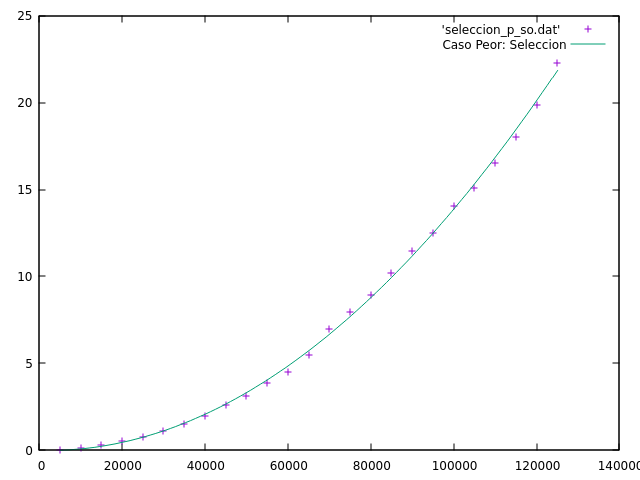
\includegraphics[scale=0.8]{seleccion_p_so_a.png}
  	\caption{Peor: Selección ajustada.}
  	
  \end{center}
\end{figure}
		
		
	\end{itemize}
	
\newpage
	
	\subsubsection{Caso Promedio}
	
	\begin{itemize}
	
		\item Análisis Empírico:
		
		\begin{table}[h]
	\begin{center}
		\begin{tabular}{|c|c|}
		\hline
		Tamaño & Tiempo \\
		\hline
		5000 & 0.026467 \\
		10000 & 0.10385 \\
		15000 & 0.231773 \\
		20000 & 0.43346 \\
		25000 & 0.664196 \\
		30000 & 0.923467 \\
		35000 & 1.31096 \\
		40000 & 1.65418 \\
		45000 & 2.07659 \\
		50000 & 2.5511 \\
		55000 & 3.21866 \\
		60000 & 3.68538 \\
		65000 & 4.31529 \\
		70000 & 5.27242 \\
		75000 & 5.8648 \\
		80000 & 6.59147 \\
		85000 & 8.32133 \\
		90000 & 9.5113 \\
		95000 & 10.9703 \\
		100000 & 11.1657 \\
		105000 & 12.108 \\
		110000 & 13.3961 \\
		115000 & 14.6338 \\
		120000 & 15.9557 \\
		125000 & 17.3286 \\
		\hline
		\end{tabular}
	\end{center}
	\caption{Algoritmo Selección en caso promedio.}
\end{table}
\newpage
		
		\item Análisis Híbrido:
		
\begin{figure}[h]
  \begin{center}
  
  	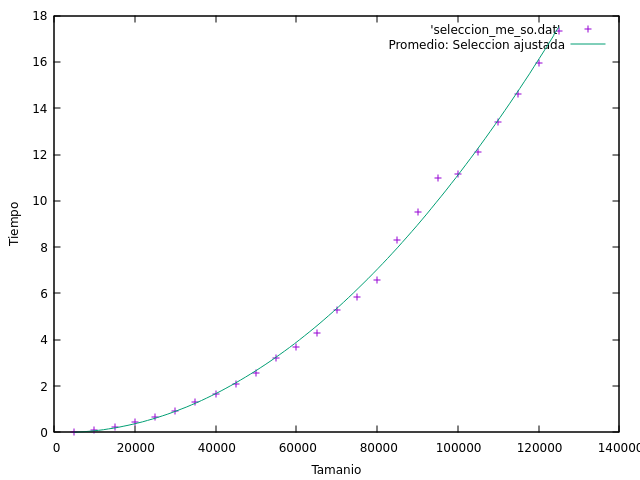
\includegraphics[scale=0.8]{seleccion_me_so_a.png}
  	\caption{Promedio: Selección ajustada.}
  	
  \end{center}
\end{figure}
		
	\end{itemize}
	\newpage
	
	\subsubsection{Caso Mejor}
	
	\begin{itemize}
	\item Análisis Empírico
	
	\begin{table}[h]
	\begin{center}
		\begin{tabular}{|c|c|}
		\hline
		Tamaño & Tiempo \\
		\hline
		5000 & 0.024232 \\
		10000 & 0.092074 \\
		15000 & 0.208886 \\
		20000 & 0.425204 \\
		25000 & 0.588021 \\
		30000 & 0.826999 \\
		35000 & 1.16475 \\
		40000 & 1.65811 \\
		45000 & 2.10846 \\
		50000 & 2.5965 \\
		55000 & 3.00598 \\
		60000 & 3.5108 \\
		65000 & 4.19494 \\
		70000 & 4.57465 \\
		75000 & 5.08036 \\
		80000 & 5.78989 \\
		85000 & 6.53294 \\
		90000 & 7.96791 \\
		95000 & 11.512 \\
		100000 & 10.6751 \\
		105000 & 11.1382 \\
		110000 & 12.0398 \\
		115000 & 13.882 \\
		120000 & 14.539 \\
		125000 & 15.2915 \\

		\hline
		\end{tabular}
	\end{center}
	\caption{Algoritmo Selección en caso mejor.}
\end{table}
\newpage
	
	\item Análisis Híbrido
	
\begin{figure}[h]
  \begin{center}
  
  	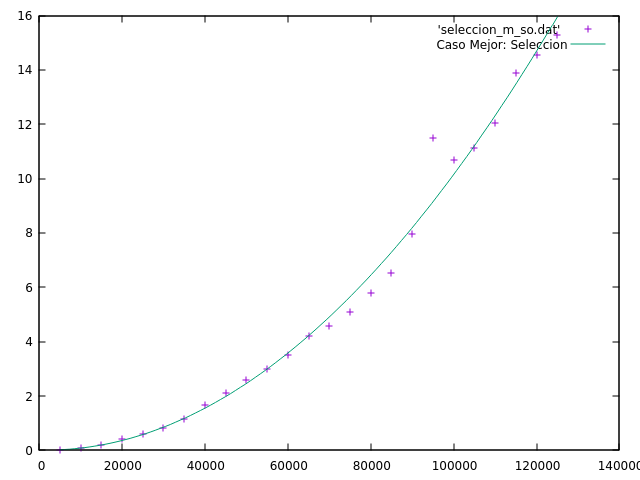
\includegraphics[scale=0.8]{seleccion_m_so_a.png}
  	\caption{Mejor: Selección ajustada.}
  	
  \end{center}
\end{figure}
	
	
	\end{itemize}
	
	
	
	
	%Algoritmos O(n*log_2(n))
\newpage
\section{Algoritmos $\textit{O(nlog(n))}$}

Por lo general, los casos peores ocurren cuando se debe ordenar un vector cuyos elementos se encuentran en orden opuesto al criterio de ordenación, los casos promedio cuando los valores se encuentran de forma aleatoria, y los casos mejores cuando el vector ya está ordenado. La única excepción es el algoritmo Quicksort, cuyo caso peor ocurre cuando el vector se encuentra ordenado, y el promedio y mejor caso cuando los elementos del vector se encuentran en él de forma aleatoria.
\newpage

\subsection{Heapsort}

	\subsubsection{Peor Caso}
	\begin{itemize}
	
		\item Análisis Teórico:
		
		\lstset{language=C++}
	\begin{lstlisting}
	
static void heapsort(double T[], int num_elem)
{
  int i;
  for (i = num_elem/2; i >= 0; i--)	//O(n)
    reajustar(T, num_elem, i);		//O(log(n))
  for (i = num_elem - 1; i >= 1; i--)	//O(n)
    {
      double aux = T[0];	//O(1)
      T[0] = T[i];
      T[i] = aux;
      reajustar(T, i, 0);	//O(log(n))
    }
}
  

static void reajustar(double T[], int num_elem, int k)
{
  int j;
  double v;
  v = T[k];
  bool esAPO = false;
  while ((k < num_elem/2) && !esAPO)	//O(log(n))
    {
      j = k + k + 1; 		//Resto O(1)
      if ((j < (num_elem - 1)) && (T[j] < T[j+1])) 
	j++;
      if (v >= T[j]){
	esAPO = true;
      }else{
      T[k] = T[j];
      k = j;
      }
    }
  T[k] = v;
}

	\end{lstlisting}
		
		Vemos que el método \textit{reajustar} es de orden logarítmico, pues su bucle interno realiza la mitad de iteraciones cada vez que se llama a la función en un bucle lineal. Por tanto, $T(n) \in O(n \log{(n)})$.
		\item Análisis Empírico:
		
		\begin{table}[h]
	\begin{center}
		\begin{tabular}{|c|c|}
		\hline
		Tamaño & Tiempo \\
		\hline
		50000 & 0.00507379 \\
		100000 & 0.00985907 \\
		150000 & 0.0150399 \\
		200000 & 0.0192911 \\
		250000 & 0.0258017 \\
		300000 & 0.0302678 \\
		350000 & 0.0359918 \\
		400000 & 0.0420974 \\
		450000 & 0.0497874 \\
		500000 & 0.0538607 \\
		550000 & 0.0599765 \\
		600000 & 0.0644207 \\
		650000 & 0.0699733 \\
		700000 & 0.0755958 \\
		750000 & 0.0806598 \\
		800000 & 0.0897942 \\
		850000 & 0.0933454 \\
		900000 & 0.0977625 \\
		950000 & 0.102721 \\
		1000000 & 0.110783 \\
		1050000 & 0.115308 \\
		1100000 & 0.121918 \\
		1150000 & 0.127592 \\
		1200000 & 0.136058 \\
		1250000 & 0.141206 \\
		\hline
		\end{tabular}
	\end{center}
	\caption{Algoritmo Heapsort en caso peor.}
\end{table}
\newpage
		
		\item Análisis Híbrido:
		
\begin{figure}[h]
  \begin{center}
  
  	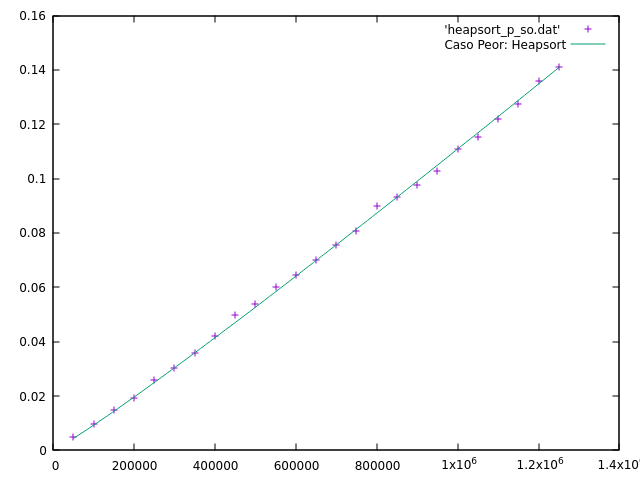
\includegraphics[scale=0.8]{heapsort_p_so_a.png}
  	\caption{Peor: Heapsort ajustado.}
  	
  \end{center}
\end{figure}
		
	\end{itemize}
\newpage
	
	\subsubsection{Caso Promedio}
	
	\begin{itemize}
		\item Análisis Empírico:
		
\begin{table}[h]
	\begin{center}
		\begin{tabular}{|c|c|}
		\hline
		Tamaño & Tiempo \\
		\hline
		50000 & 0.00644205 \\
		100000 & 0.0145059 \\
		150000 & 0.0223693 \\
		200000 & 0.0324643 \\
		250000 & 0.0396175 \\
		300000 & 0.0472015 \\
		350000 & 0.0563585 \\
		400000 & 0.0657466 \\
		450000 & 0.074766 \\
		500000 & 0.0826303 \\
		550000 & 0.0945916 \\
		600000 & 0.103885 \\
		650000 & 0.11778 \\
		700000 & 0.120016 \\
		750000 & 0.133508 \\
		800000 & 0.141793 \\
		850000 & 0.150194 \\
		900000 & 0.162711 \\
		950000 & 0.173837 \\
		1000000 & 0.181508 \\
		1050000 & 0.194676 \\
		1100000 & 0.20109 \\
		1150000 & 0.212023 \\
		1200000 & 0.222133 \\
		1250000 & 0.235588 \\
		\hline
		\end{tabular}
	\end{center}
	\caption{Algoritmo Heapsort en caso promedio.}
\end{table}
\newpage
		
		\item Análisis Híbrido:
		
\begin{figure}[h]
  \begin{center}
  
  	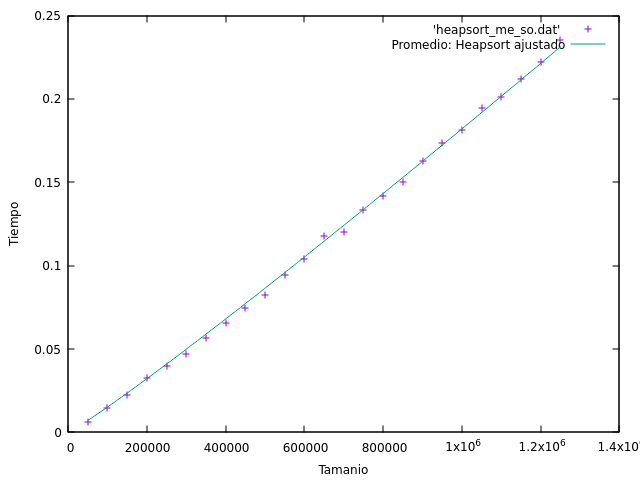
\includegraphics[scale=0.8]{heapsort_me_so_a.png}
  	\caption{Promedio: Heapsort ajustado.}
  	
  \end{center}
\end{figure}
		
		
	\end{itemize}
\newpage
	
	\subsubsection{Caso Mejor}
	
	\begin{itemize}
	\item Análisis Empírico
	
	\begin{table}[h]
	\begin{center}
		\begin{tabular}{|c|c|}
		\hline
		Tamaño & Tiempo \\
		\hline
		50000 & 0.00492359 \\ 
		100000 & 0.00956164 \\
		150000 & 0.0156657 \\ 
		200000 & 0.01963 \\ 
		250000 & 0.0243095 \\ 
		300000 & 0.0313337 \\ 
		350000 & 0.0396175 \\ 
		400000 & 0.0482821 \\ 
		450000 & 0.0461801 \\ 
		500000 & 0.0576095 \\ 
		550000 & 0.0592529 \\ 
		600000 & 0.0624077 \\ 
		650000 & 0.068794 \\ 
		700000 & 0.0727778 \\ 
		750000 & 0.0813073 \\ 
		800000 & 0.0856724 \\ 
		850000 & 0.0912698 \\ 
		900000 & 0.0992181 \\ 
		950000 & 0.099018 \\ 
		1000000 & 0.104945 \\ 
		1050000 & 0.128995 \\ 
		1100000 & 0.120285 \\ 
		1150000 & 0.131505 \\ 
		1200000 & 0.134781 \\ 
		1250000 & 0.13407 \\
		\hline
		\end{tabular}
	\end{center}
	\caption{Algoritmo Heapsort en caso mejor.}
\end{table}
\newpage
	
	\item Análisis Híbrido
	
\begin{figure}[h]
  \begin{center}
  
  	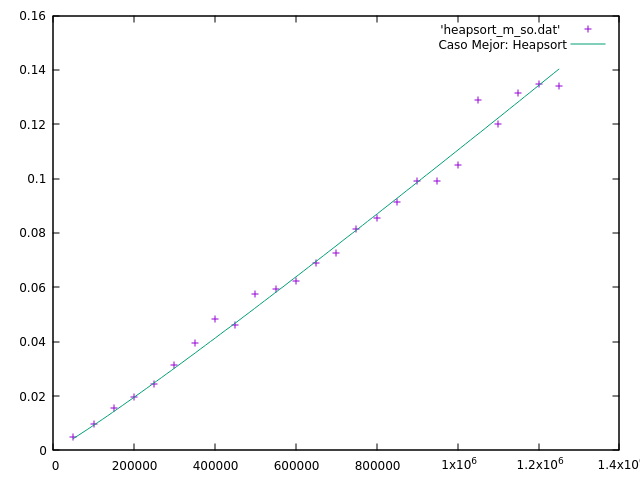
\includegraphics[scale=0.8]{heapsort_m_so_a.png}
  	\caption{Mejor: Heapsort ajustado.}
  	
  \end{center}
\end{figure}
	
	
	\end{itemize}
\newpage
	
	

\subsection{Mergesort}

	\subsubsection{Peor Caso}
	\begin{itemize}
	
		\item Análisis Teórico:
		
		\lstset{language=C++}
	\begin{lstlisting}
	
void mergesort(double T[], int num_elem)
{
  mergesort_lims(T, 0, num_elem);
}

static void mergesort_lims(double T[], int inicial, int final)
{
  if (final - inicial < UMBRAL_MS)
    {
      insercion_lims(T, inicial, final); //Dado que se utiliza
      					//para tamanios 
      					//de vector 
      					//relativamente 
      					//pequenios,  
      					//no se considera 
      					//para caso peor.
    } else {
      int k = (final - inicial)/2;

      double * U = new double [k - inicial + 1];
      assert(U);
      int l, l2;
      for (l = 0, l2 = inicial; l < k; l++, l2++)	//O(n)
	U[l] = T[l2];
      U[l] = INT_MAX;

      double * V = new double [final - k + 1];
      assert(V);
      for (l = 0, l2 = k; l < final - k; l++, l2++)
	V[l] = T[l2];
      V[l] = INT_MAX;

      mergesort_lims(U, 0, k);
      mergesort_lims(V, 0, final - k);
      fusion(T, inicial, final, U, V);	//O(n)
      delete [] U;
      delete [] V;
    };
}
  

static void fusion(double T[], int inicial, int final, 
		double U[], double V[])
{
  int j = 0;
  int k = 0;
  for (int i = inicial; i < final; i++)	//O(n)
    {
      if (U[j] < V[k]) {	//Resto O(1)
	T[i] = U[j];
	j++;
      } else{
	T[i] = V[k];
	k++;
      };
    };
}

	\end{lstlisting}
	
	 Vemos que tanto la función \textit{fusión} como los bucles internos son de orden lineal. Sin embargo, debemos darnos cuenta que la variable de control \textit{k} se reduce a la mitad en cada llamada recursiva. Por tanto, se ejecuta una instrucción lineal un número logarítmico de veces, es decir, $T(n) \in O(n \log{(n)})$
	 
\newpage
	 
		\item Análisis Empírico:
		
		\begin{table}[h]
	\begin{center}
		\begin{tabular}{|c|c|}
		\hline
		Tamaño & Tiempo \\
		\hline
		50000 & 0.010584 \\
		100000 & 0.021168 \\
		150000 & 0.026842 \\
		200000 & 0.043895 \\
		250000 & 0.042136 \\
		300000 & 0.055757 \\
		350000 & 0.07173 \\
		400000 & 0.089655 \\
		450000 & 0.071658 \\
		500000 & 0.083383 \\
		550000 & 0.098574 \\
		600000 & 0.114057 \\
		650000 & 0.129123 \\
		700000 & 0.14452 \\
		750000 & 0.181274 \\
		800000 & 0.182727 \\
		850000 & 0.137131 \\
		900000 & 0.147268 \\
		950000 & 0.181828 \\
		1000000 & 0.172762 \\
		1050000 & 0.189469 \\
		1100000 & 0.201065 \\
		1150000 & 0.217483 \\
		1200000 & 0.230875 \\
		1250000 & 0.246414 \\
		\hline
		\end{tabular}
	\end{center}
	\caption{Algoritmo Mergesort en caso peor.}
\end{table}
\newpage
		
		
		\item Análisis Híbrido:
		
\begin{figure}[h]
  \begin{center}
  
  	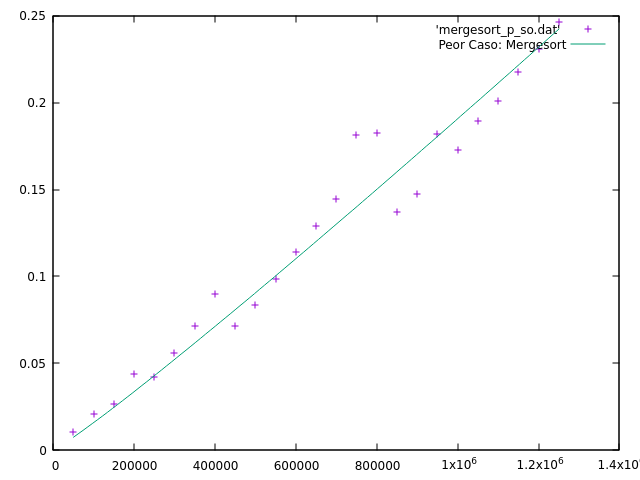
\includegraphics[scale=0.8]{mergesort_p_so_a.png}
  	\caption{Peor: Mergesort ajustado.}
  	
  \end{center}
\end{figure}
		
		
		
	\end{itemize}
\newpage
	
	\subsubsection{Caso Promedio}
	\begin{itemize}
	
		\item Análisis Empírico:
		
\begin{table}[h]
	\begin{center}
		\begin{tabular}{|c|c|}
		\hline
		Tamaño & Tiempo \\
		\hline
		50000 & 0.008737 \\	
		100000 & 0.018508 \\	
		150000 & 0.026026 \\	
		200000 & 0.037912 \\	
		250000 & 0.043089 \\	
		300000 & 0.053945 \\	
		350000 & 0.06879 \\	
		400000 & 0.084573 \\	
		450000 & 0.112725 \\	
		500000 & 0.092512 \\	
		550000 & 0.103397 \\	
		600000 & 0.120889 \\	
		650000 & 0.127054 \\	
		700000 & 0.140146 \\	
		750000 & 0.156702 \\	
		800000 & 0.171457 \\	
		850000 & 0.159553 \\	
		900000 & 0.170878 \\	
		950000 & 0.177797 \\	
		1000000 & 0.188466 \\	
		1050000 & 0.202553 \\	
		1100000 & 0.213601 \\	
		1150000 & 0.226186 \\	
		1200000 & 0.238423 \\	
		1250000 & 0.252582 \\	
		\hline
		\end{tabular}
	\end{center}
	\caption{Algoritmo Mergesort en caso promedio.}
\end{table}
\newpage
		
		\item Análisis Híbrido:
		
\begin{figure}[h]
  \begin{center}
  
  	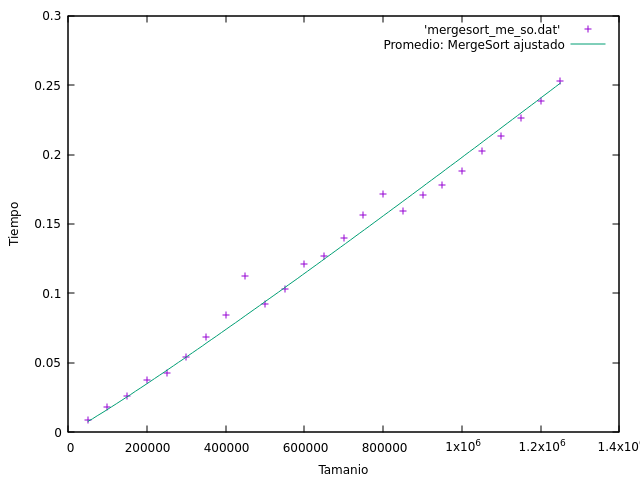
\includegraphics[scale=0.8]{mergesort_me_so_a.png}
  	\caption{Promedio: Mergesort ajustado.}
  	
  \end{center}
\end{figure}
		
	\end{itemize}
	\newpage
	
	
	\subsubsection{Caso Mejor}
	
	\begin{itemize}
	\item Análisis Empírico
	
	\begin{table}[h]
	\begin{center}
		\begin{tabular}{|c|c|}
		\hline
		Tamaño & Tiempo \\
		\hline
		50000 & 0.003102 \\
		100000 & 0.006945 \\
		150000 & 0.010423 \\
		200000 & 0.01447 \\
		250000 & 0.018185 \\
		300000 & 0.022385 \\
		350000 & 0.026579 \\
		400000 & 0.03091 \\
		450000 & 0.034869 \\
		500000 & 0.040476 \\
		550000 & 0.045227 \\
		600000 & 0.05317 \\
		650000 & 0.058028 \\
		700000 & 0.064596 \\
		750000 & 0.068245 \\
		800000 & 0.07343 \\
		850000 & 0.075668 \\
		900000 & 0.075407 \\
		950000 & 0.079859 \\
		1000000 & 0.084735 \\
		1050000 & 0.089942 \\
		1100000 & 0.095477 \\
		1150000 & 0.098606 \\
		1200000 & 0.107842 \\
		1250000 & 0.108601 \\
		\hline
		\end{tabular}
	\end{center}
	\caption{Algoritmo Mergesort en caso mejor.}
\end{table}
\newpage
	
	\item Análisis Híbrido
\begin{figure}[h]
  \begin{center}
  
  	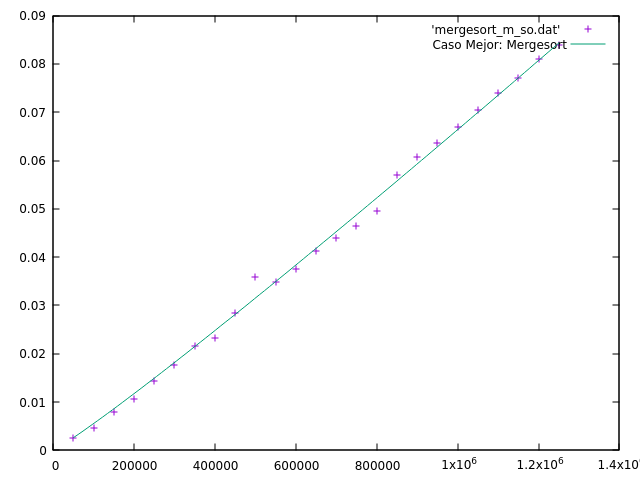
\includegraphics[scale=0.8]{mergesort_m_so_a.png}
  	\caption{Mejor: MergeSort ajustado.}
  	
  \end{center}
\end{figure}
	
	\end{itemize}
	
\newpage

	

\subsection{Quicksort}

	\subsubsection{Peor Caso}
	\begin{itemize}
	
		\item Análisis Teórico: 
		
		\lstset{language=C++}
	\begin{lstlisting}
	
inline static void insercion(double T[], int num_elem)
{
  insercion_lims(T, 0, num_elem);
}


static void insercion_lims(double T[], int inicial, int final)
{
  int i, j;
    double aux;
  for (i = inicial + 1; i < final; i++) {
    j = i;
    while ((T[j] < T[j-1]) && (j > 0)) {
      aux = T[j];
      T[j] = T[j-1];
      T[j-1] = aux;
      j--;
    };
  };
}


const int UMBRAL_QS = 50;


inline void quicksort(double T[], int num_elem)
{
  quicksort_lims(T, 0, num_elem);
}

static void quicksort_lims(double T[], int inicial, int final)
{
  int k;
  if (final - inicial < UMBRAL_QS) {	//Casos pequenios que
    insercion_lims(T, inicial, final);	//no tenemos en cuenta
    					
  } else {
    dividir_qs(T, inicial, final, k);
    quicksort_lims(T, inicial, k);
    quicksort_lims(T, k + 1, final);
  };
}


static void dividir_qs(double T[], int inicial, int final, 
			int & pp)
{
  double pivote, aux;
  int k, l;

  pivote = T[inicial];
  k = inicial;
  l = final;
  do {
    k++;
  } while ((T[k] <= pivote) && (k < final-1));	//O(n)
  do {
    l--;
  } while (T[l] > pivote);		//O(n)
  while (k < l) {			//O(n)
    aux = T[k];
    T[k] = T[l];
    T[l] = aux;
    do k++; while (T[k] <= pivote);
    do l--; while (T[l] > pivote);
  };
  aux = T[inicial];			//O(1)
  T[inicial] = T[l];
  T[l] = aux;
  pp = l;
};

	\end{lstlisting}
	
\newpage

	Al llamar a cada submitad del vector, y sumando \textit{dividir\_qs}, se tiene que $T(n)=2T(\frac{n}{2}) + n $. 
	
	Resolviendo la ecuación de recurrencias:\\
	$T(n)= c_1 \cdot n + c_2 \cdot n \log{(n)}, c_1,c_2 \in \mathbb{R^+} \Rightarrow T(n) \in O(n \log{(n)})$
	
	
		\item Análisis Empírico:
		
\begin{table}[h]
	\begin{center}
		\begin{tabular}{|c|c|}
		\hline
		Tamaño & Tiempo \\
		\hline
		5000 & 0.0220869 \\
		10000 & 0.0849181 \\
		15000 & 0.188108 \\
		20000 & 0.334722 \\
		25000 & 0.526816 \\
		30000 & 0.747888 \\
		35000 & 1.03453 \\
		40000 & 1.33098 \\
		45000 & 1.68591 \\
		50000 & 2.11947 \\
		55000 & 2.54125 \\
		60000 & 3.04818 \\
		65000 & 3.95525 \\
		70000 & 4.16632 \\
		75000 & 5.2601 \\
		80000 & 5.94749 \\
		85000 & 6.07466 \\
		90000 & 6.89523 \\
		95000 & 7.60161 \\
		100000 & 8.5458 \\
		105000 & 9.2701 \\
		110000 & 10.3675 \\
		115000 & 11.1341 \\
		120000 & 12.3011 \\
		125000 & 13.2399 \\
		\hline
		\end{tabular}
	\end{center}
	\caption{Algoritmo Quicksort en caso peor.}
\end{table}

\newpage
		
		\item Análisis Híbrido:
		
\begin{figure}[h]
  \begin{center}
  
  	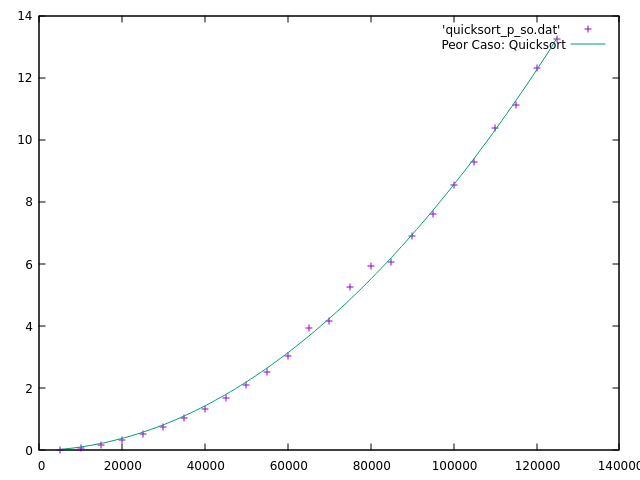
\includegraphics[scale=0.8]{quicksort_p_so_a.png}
  	\caption{Peor: Quicksort ajustado. Podemos apreciar que el ajuste ronda lo cuadrático.}
  	
  \end{center}
\end{figure}
		
	\end{itemize}


	
\newpage
	
	\subsubsection{Caso Promedio}
	
	\begin{itemize}
	
		\item Análisis Empírico:
		
\begin{table}[h]
	\begin{center}
		\begin{tabular}{|c|c|}
		\hline
		Tamaño & Tiempo \\
		\hline
		50000 & 0.00526966 \\
		100000 & 0.0111132 \\
		150000 & 0.0170174 \\
		200000 & 0.0239087 \\
		250000 & 0.0293342 \\
		300000 & 0.035813 \\
		350000 & 0.0423003 \\
		400000 & 0.0500287 \\
		450000 & 0.056987 \\
		500000 & 0.0622721 \\
		550000 & 0.0685469 \\
		600000 & 0.0763339 \\
		650000 & 0.0825871 \\
		700000 & 0.0904075 \\
		750000 & 0.0955742 \\
		800000 & 0.104228 \\
		850000 & 0.110338 \\
		900000 & 0.117366 \\
		950000 & 0.124273 \\
		1000000 & 0.129478 \\
		1050000 & 0.141046 \\
		1100000 & 0.144929 \\
		1150000 & 0.153193 \\
		1200000 & 0.159648 \\
		1250000 & 0.167178 \\
		\hline
		\end{tabular}
	\end{center}
	\caption{Algoritmo Quicksort en caso promedio.}
\end{table}
\newpage
		
		\item Análisis Híbrido:
\begin{figure}[h]
  \begin{center}
  
  	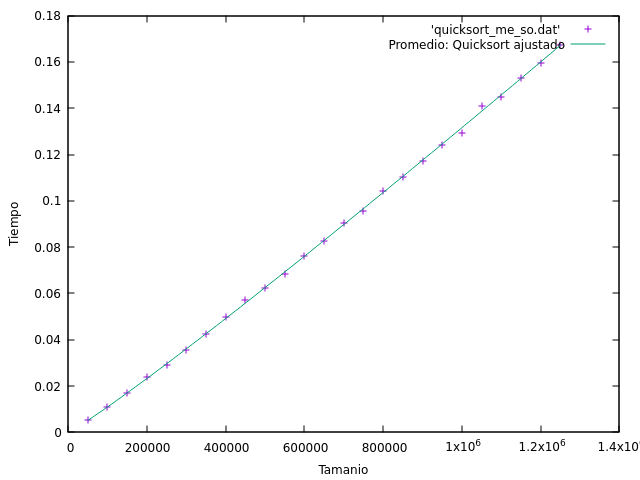
\includegraphics[scale=0.8]{quicksort_me_so_a.png}
  	\caption{Promedio: Quicksort ajustado.}
  	
  \end{center}
\end{figure}
		
	\end{itemize}
	\newpage
	
	\subsubsection{Caso Mejor}
	
	\begin{itemize}
	\item Análisis Empírico
	
	\begin{table}[h]
	\begin{center}
		\begin{tabular}{|c|c|}
		\hline
		Tamaño & Tiempo \\
		\hline
		50000 & 0.002568 \\
		100000 & 0.004726 \\
		150000 & 0.007874 \\
		200000 & 0.010547 \\
		250000 & 0.014276 \\
		300000 & 0.017682 \\
		350000 & 0.021711 \\
		400000 & 0.023303 \\
		450000 & 0.028501 \\
		500000 & 0.035828 \\
		550000 & 0.034852 \\
		600000 & 0.037527 \\
		650000 & 0.041249 \\
		700000 & 0.043925 \\
		750000 & 0.04641 \\
		800000 & 0.049579 \\
		850000 & 0.056985 \\
		900000 & 0.060708 \\
		950000 & 0.063535 \\
		1000000 & 0.066879 \\
		1050000 & 0.070372 \\
		1100000 & 0.074037 \\
		1150000 & 0.076987 \\
		1200000 & 0.081046 \\
		1250000 & 0.083857 \\
		\hline
		\end{tabular}
	\end{center}
	\caption{Algoritmo Quicksort en caso mejor.}
\end{table}
\newpage

	
	\item Análisis Híbrido
	
\begin{figure}[h]
  \begin{center}
  
  	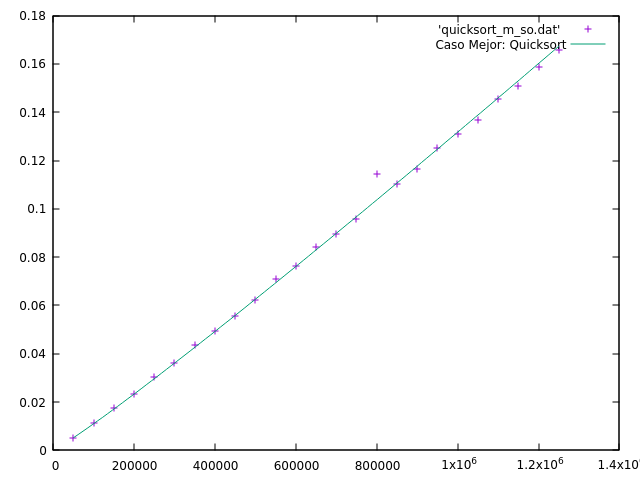
\includegraphics[scale=0.8]{quicksort_m_so_a.png}
  	\caption{Mejor: Quicksort ajustado.}
  	
  \end{center}
\end{figure}
	
	
	\end{itemize}
	
\newpage
	%Eficiencia variando la compilacion	
	\section{Eficiencia Empírica con variación de parámetros externos}
	
	El análisis empírico puede verse influido por factores externos como el modelo de computador, el sistema operativo, las opciones de compilación, etc. Nos centraremos en estudiar esta variación debido a la compilación con optimización. Para ello, utilizamos la opción de compilación con optimización más agresiva:\\
	
\fbox{\textbf{g++ \textit{nombre.cpp} -o \textit{nombre} -O3}.}
\newpage


	\subsection{Burbuja}
	
\begin{itemize}
	
	\item Análisis empírico.
	
\begin{table}[h]
	\begin{center}
		\begin{tabular}{|c|c|}
		\hline
		Tamaño & Tiempo \\
		\hline
		5000 & 0.0377814 \\
		10000 & 0.146614 \\
		15000 & 0.424735 \\
		20000 & 0.715906 \\
		25000 & 1.14998 \\
		30000 & 1.7023 \\
		35000 & 2.31612 \\
		40000 & 3.46276 \\
		45000 & 4.44725 \\
		50000 & 5.54374 \\
		55000 & 6.46876 \\
		60000 & 7.31685 \\
		65000 & 8.57751 \\
		70000 & 9.7199 \\
		75000 & 11.2378 \\
		80000 & 12.9095 \\
		85000 & 15.0907 \\
		90000 & 16.2756 \\
		95000 & 17.9327 \\
		100000 & 20.3645 \\
		105000 & 23.4413 \\
		110000 & 24.2647 \\
		115000 & 26.8178 \\
		120000 & 29.1067 \\
		125000 & 31.7164 \\
		\hline
		\end{tabular}
	\end{center}
	\caption{Promedio: Burbuja con optimización.}
\end{table}

\newpage

\begin{figure}[h]
  \begin{center}
  
  	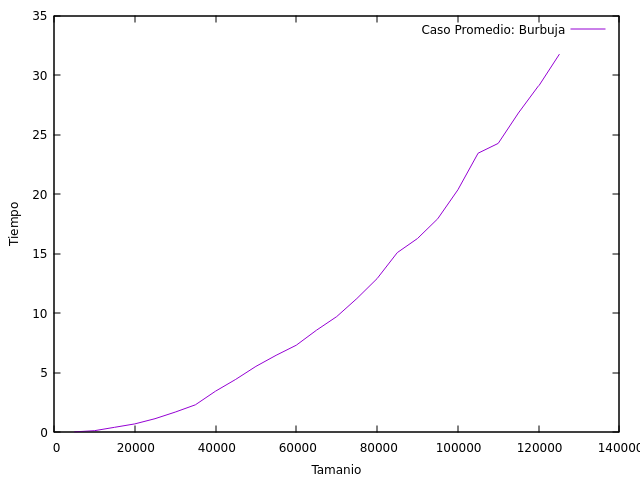
\includegraphics[scale=0.8]{burbuja_me_co.png}
  	\caption{Burbuja con optimización.}
  	
  \end{center}
\end{figure}

\newpage
	
\end{itemize}
	
	
	\subsection{Inserción}
	
\begin{itemize}
	
	\item Análisis empírico.
	
\begin{table}[h]
	\begin{center}
		\begin{tabular}{|c|c|}
		\hline
		Tamaño & Tiempo \\
		\hline
		5000 & 0.0176335 \\
		10000 & 0.0666303 \\
		15000 & 0.14557 \\
		20000 & 0.27043 \\
		25000 & 0.413972 \\
		30000 & 0.583728 \\
		35000 & 0.798968 \\
		40000 & 1.05335 \\
		45000 & 1.55234 \\
		50000 & 1.83778 \\
		55000 & 2.23658 \\
		60000 & 2.66345 \\
		65000 & 3.11851 \\
		70000 & 3.60326 \\
		75000 & 4.15626 \\
		80000 & 4.44012 \\
		85000 & 5.11374 \\
		90000 & 5.4513 \\
		95000 & 5.8375 \\
		100000 & 6.50648 \\
		105000 & 7.1411 \\
		110000 & 7.90262 \\
		115000 & 8.70768 \\
		120000 & 9.72115 \\
		125000 & 10.4252 \\
		\hline
		\end{tabular}
	\end{center}
	\caption{Promedio: Inserción con optimización.}
\end{table}
\newpage

\begin{figure}[h]
  \begin{center}
  
  	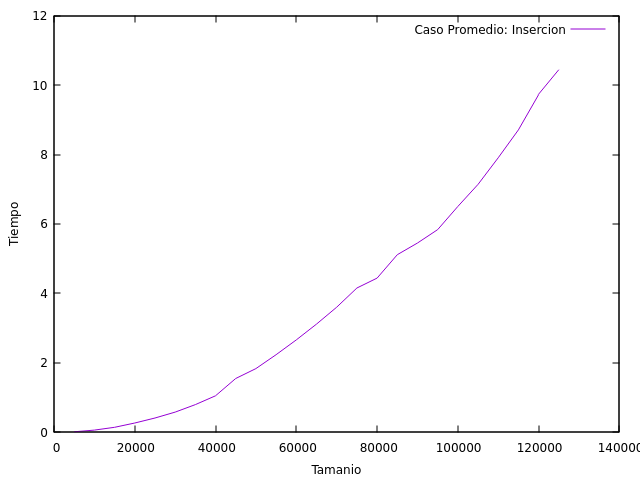
\includegraphics[scale=0.8]{insercion_me_co.png}
  	\caption{Inserción con optimización.}
  	
  \end{center}
\end{figure}
	
\end{itemize}
\newpage
	
	\subsection{Selección}
	
\begin{itemize}
	
	\item Análisis empírico.
	
\begin{table}[h]
	\begin{center}
		\begin{tabular}{|c|c|}
		\hline
		Tamaño & Tiempo \\
		\hline
		5000 & 0.003615 \\
		10000 & 0.013605 \\
		15000 & 0.029302 \\
		20000 & 0.051696 \\
		25000 & 0.080692 \\
		30000 & 0.113846 \\
		35000 & 0.155257 \\
		40000 & 0.202168 \\
		45000 & 0.256989 \\
		50000 & 0.312794 \\
		55000 & 0.379782 \\
		60000 & 0.448623 \\
		65000 & 0.529456 \\
		70000 & 0.610602 \\
		75000 & 0.702361 \\
		80000 & 0.817145 \\
		85000 & 0.931516 \\
		90000 & 1.02283 \\
		95000 & 1.12776 \\
		100000 & 1.25124 \\
		105000 & 1.37287 \\
		110000 & 1.5067 \\
		115000 & 1.63886 \\
		120000 & 1.7874 \\
		125000 & 2.00971 \\
		\hline
		\end{tabular}
	\end{center}
	\caption{Promedio: Selección con optimización.}
\end{table}
\newpage

\begin{figure}[h]
  \begin{center}
  
  	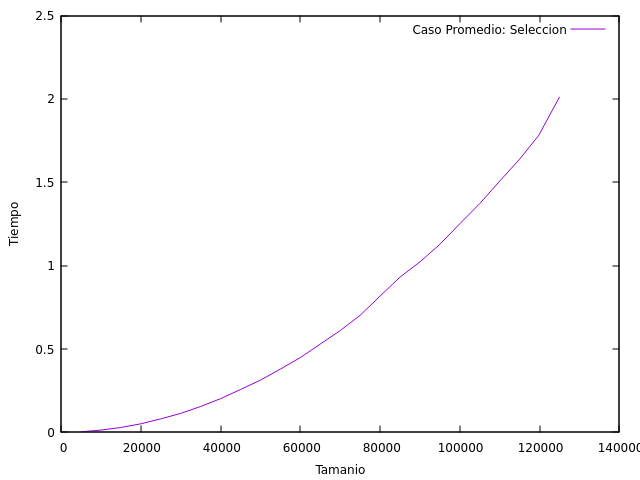
\includegraphics[scale=0.8]{seleccion_me_co.png}
  	\caption{Selección con optimización.}
  	
  \end{center}
\end{figure}

\newpage
	
\end{itemize}
	
	\subsection{Heapsort}
	
\begin{itemize}
	
	\item Análisis empírico.
\begin{table}[h]
	\begin{center}
		\begin{tabular}{|c|c|}
		\hline
		Tamaño & Tiempo \\
		\hline
		50000 & 0.00412993 \\
		100000 & 0.00990374 \\
		150000 & 0.01416 \\
		200000 & 0.0195406 \\
		250000 & 0.0246558 \\
		300000 & 0.0301945 \\
		350000 & 0.0359811 \\
		400000 & 0.0415768 \\
		450000 & 0.0475179 \\
		500000 & 0.053534 \\
		550000 & 0.060059 \\
		600000 & 0.0665195 \\
		650000 & 0.0742081 \\
		700000 & 0.077685 \\
		750000 & 0.0848953 \\
		800000 & 0.0908051 \\
		850000 & 0.0967343 \\
		900000 & 0.104518 \\
		950000 & 0.109678 \\
		1000000 & 0.118111 \\
		1050000 & 0.124065 \\
		1100000 & 0.132533 \\
		1150000 & 0.137528 \\
		1200000 & 0.144967 \\
		1250000 &0.153617 \\

		\hline
		\end{tabular}
	\end{center}
	\caption{Promedio: Heapsort con optimización.}
\end{table}
\newpage

\begin{figure}[h]
  \begin{center}
  
  	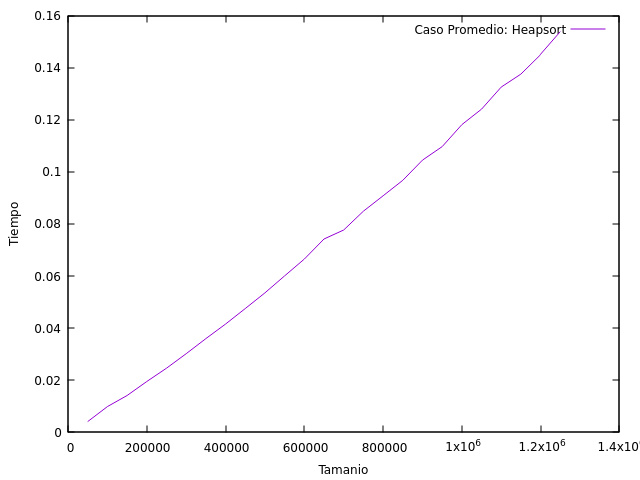
\includegraphics[scale=0.8]{heapsort_me_co.png}
  	\caption{Heapsort con optimización.}
  	
  \end{center}
\end{figure}
	
\end{itemize}
\newpage
	
	\subsection{Mergesort}
	
\begin{itemize}
	
	\item Análisis empírico.
	
\begin{table}[h]
	\begin{center}
		\begin{tabular}{|c|c|}
		\hline
		Tamaño & Tiempo \\
		\hline
		50000 & 0.003102 \\
		100000 & 0.006945 \\
		150000 & 0.010423 \\
		200000 & 0.01447 \\
		250000 & 0.018185 \\
		300000 & 0.022385 \\
		350000 & 0.026579 \\
		400000 & 0.03091 \\
		450000 & 0.034869 \\
		500000 & 0.040476 \\
		550000 & 0.045227 \\
		600000 & 0.05317 \\
		650000 & 0.058028 \\
		700000 & 0.064596 \\
		750000 & 0.068245 \\
		800000 & 0.07343 \\
		850000 & 0.075668 \\
		900000 & 0.075407 \\
		950000 & 0.079859 \\
		1000000 & 0.084735 \\
		1050000 & 0.089942 \\
		1100000 & 0.095477 \\
		1150000 & 0.098606 \\
		1200000 & 0.107842 \\
		1250000 & 0.108601 \\
		\hline
		\end{tabular}
	\end{center}
	\caption{Promedio: Mergesort con optimización.}
\end{table}
\newpage

\begin{figure}[h]
  \begin{center}
  
  	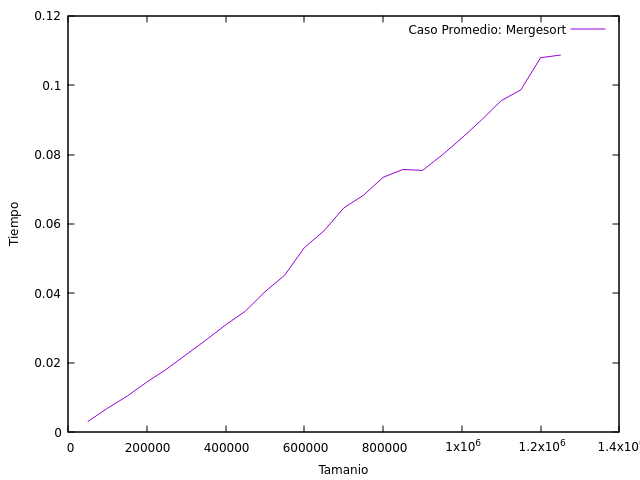
\includegraphics[scale=0.8]{mergesort_me_co.png}
  	\caption{Mergesort con optimización.}
  	
  \end{center}
\end{figure}
	
\end{itemize}
\newpage
	
	\subsection{Quicksort}
	
\begin{itemize}
	
	\item Análisis empírico.
	
\begin{table}[h]
	\begin{center}
		\begin{tabular}{|c|c|}
		\hline
		Tamaño & Tiempo \\
		\hline
		50000 & 0.00243559 \\
		100000 & 0.00532813 \\
		150000 & 0.0079174 \\
		200000 & 0.0112057 \\
		250000 & 0.0141092 \\
		300000 & 0.0169188 \\
		350000 & 0.0201969 \\
		400000 & 0.0235688 \\
		450000 & 0.0260884 \\
		500000 & 0.0292945 \\
		550000 & 0.0328711 \\
		600000 & 0.0368558 \\
		650000 & 0.0396623 \\
		700000 & 0.0420785 \\
		750000 & 0.0459312 \\
		800000 & 0.0491487 \\
		850000 & 0.0523327 \\
		900000 & 0.0561775 \\
		950000 & 0.0588771 \\
		1000000 & 0.0628896 \\
		1050000 & 0.0661846 \\
		1100000 & 0.0693547 \\
		1150000 & 0.0735047 \\
		1200000 & 0.0773954 \\
		1250000 & 0.0802944 \\
		\hline
		\end{tabular}
	\end{center}
	\caption{Promedio: Quicksort con optimización}
\end{table}
\newpage

\begin{figure}[h]
  \begin{center}
  
  	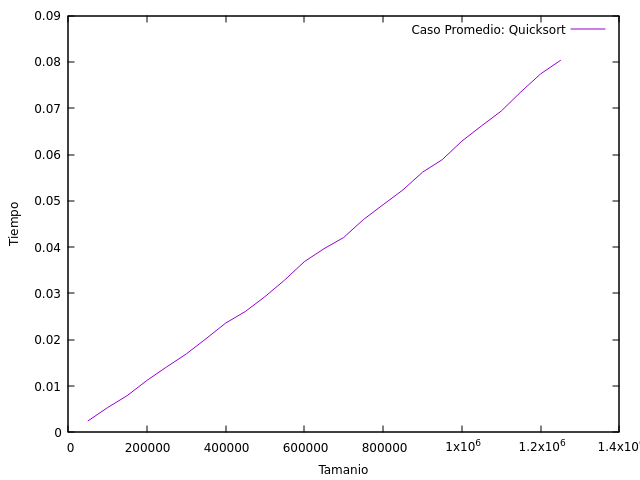
\includegraphics[scale=0.8]{quicksort_me_co.png}
  	\caption{Quicksort con optimización.}
  	
  \end{center}
\end{figure}
	
\end{itemize}
\newpage
	

\section{Comparaciones}

	Para las siguientes comparaciones se han tomado los casos promedio de los algoritmos.

	\subsection{Algoritmos $\textit{O(n²)}$}
	
	Vemos que Selección es el más eficiente y, claramente, Burbuja el menos:
	
\begin{figure}[h]
  \begin{center}
  
  	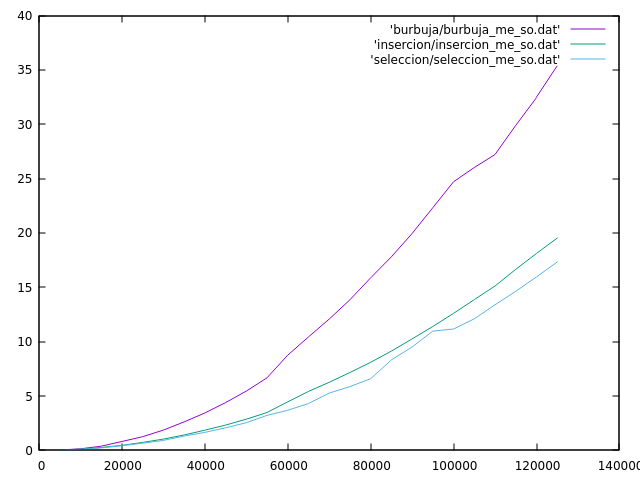
\includegraphics[scale=0.8]{comparacion_cuadraticos.png}
  	\caption{Comparación de algoritmos cuadráticos en caso promedio.}
  	
  \end{center}
\end{figure}


\newpage
	
	\subsection{Algoritmos $\textit{O(nlog(n))}$}
	
	Vemos que Quicksort es el más eficiente y Mergesort el menos, seguido de cerca por Heapsort:
	
\begin{figure}[h]
  \begin{center}
  
  	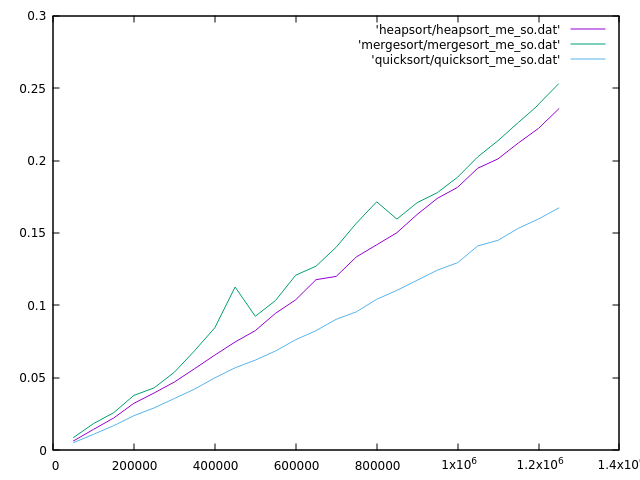
\includegraphics[scale=0.8]{comparacion_logaritmicos.png}
  	\caption{Comparación de algoritmos logarítmicos en caso promedio.}
  	
  \end{center}
\end{figure}


\newpage
	
	\subsection{Sin optimización VS Con optimización}
	
	En todos los siguientes casos podemos apreciar que la optimización supone una mejora sustancial en el tiempo de ejecución de los algoritmos.
	
	
	\subsubsection{Burbuja}
	
\begin{figure}[h]
  \begin{center}
  
  	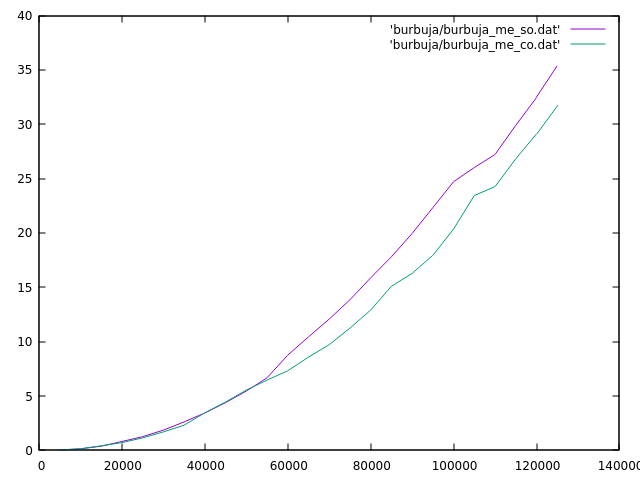
\includegraphics[scale=0.8]{comparacion_bb.png}
  	\caption{Burbuja.}
  	
  \end{center}
\end{figure}

\newpage

	\subsubsection{Inserción}

\begin{figure}[h]
  \begin{center}
  
  	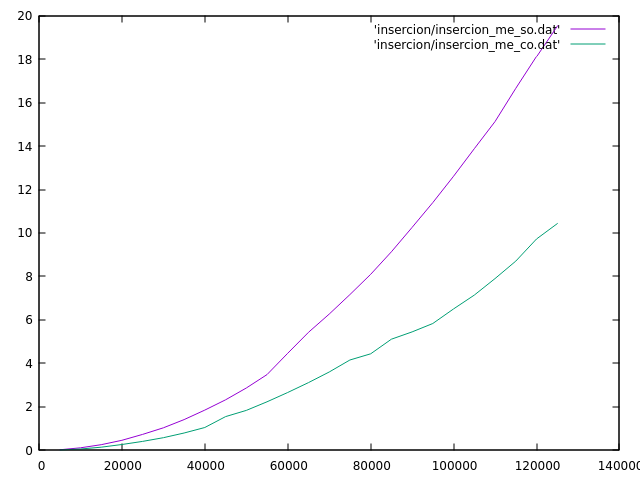
\includegraphics[scale=0.8]{comparacion_ii.png}
  	\caption{Inserción.}
  	
  \end{center}
\end{figure}


\newpage


	\subsubsection{Selección}

\begin{figure}[h]
  \begin{center}
  
  	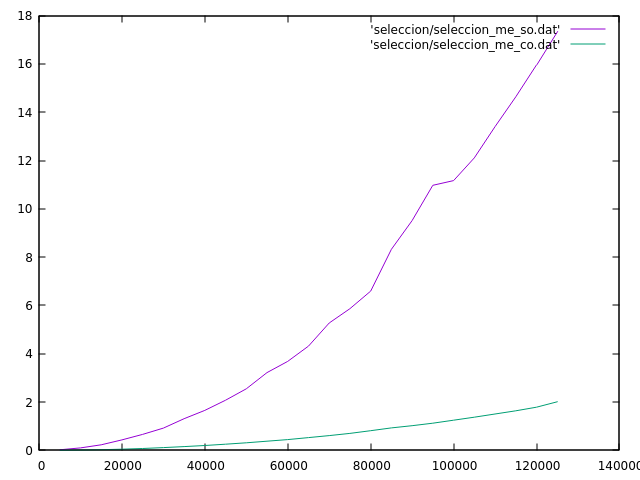
\includegraphics[scale=0.8]{comparacion_ss.png}
  	\caption{Selección.}
  	
  \end{center}
\end{figure}



\newpage
  
  	\subsubsection{Heapsort}
  	
\begin{figure}[h]
  \begin{center}
  
  	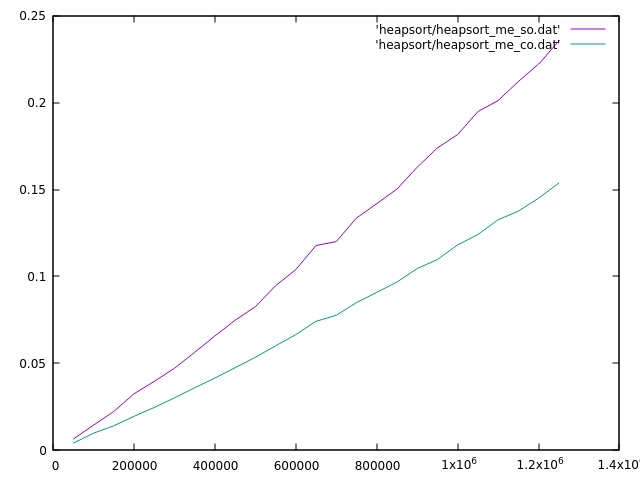
\includegraphics[scale=0.8]{comparacion_hh.png}
  	\caption{Heapsort.}
  	
  \end{center}
\end{figure}

\newpage

	\subsubsection{Mergesort}

\begin{figure}[h]
  \begin{center}
  
  	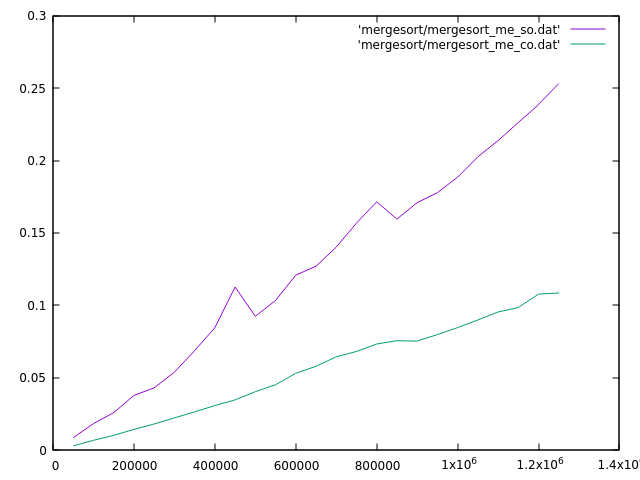
\includegraphics[scale=0.8]{comparacion_mm.png}
  	\caption{Mergesort.}
  	
  \end{center}
\end{figure}

\newpage

	\subsubsection{Quicksort}

\begin{figure}[h]
  \begin{center}
  
  	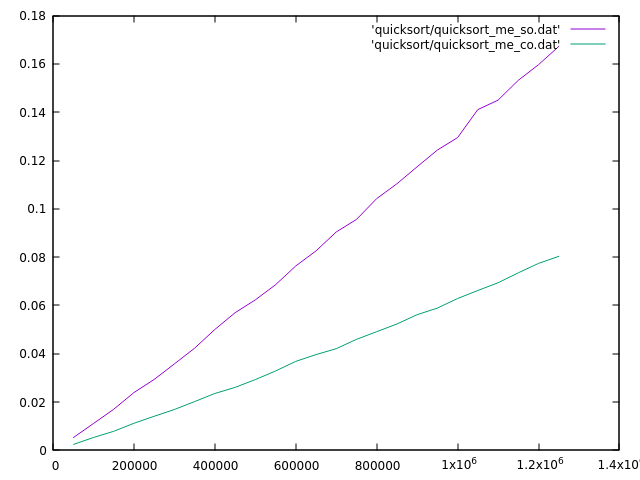
\includegraphics[scale=0.8]{comparacion_qq.png}
  	\caption{Quicksort.}
  	
  \end{center}
\end{figure}

	
\newpage


\section{Conclusiones}

Como conclusiones importantes que se extraen de esta práctica destacan:

\begin{itemize}
	\item La importancia del análisis teórico para determinar si de verdad es rentable implementar un algoritmo.
	\item La importancia del análisis híbrido para confirmar el análisis teórico.
	\item La importancia de la optimización en cuanto a la reducción de tiempo de ejecución.
	\item Cómo las diferentes notaciones de eficiencia permiten determinar la mejor opción a utilizar según el tamaño y condición de los datos a ordenar.
\end{itemize}


\end{document}